\begin{center} 
\emph{``Life is a mirror and will reflect back to the thinker what he thinks into it.'' --  Ernest Holmes}
\end{center}

\section{Linear Transformations on $\R^2$}\label{sec:trans2}
In this section, we will explore how multiplication by a nonsingular matrix transforms geometry in $\R^2$. While analogous statements can be extended to the vector space $F^n$, based upon the field $F$ itself, only some geometric interpretations may apply.\\

Let $a, b\in \R$ such that $a,b > 0$. \vspace{-0.1 in}
\begin{multicols}{2}
\noindent We can \textbf{stretch} $\R^2$ \textbf{horizontally} by multiplying the (scaling) matrix 
\[\mtx{rr}{a&0\\0&1}.\] 
\noindent We can \textbf{stretch} $\R^2$ \textbf{vertically} by multiplying the matrix 
\[\mtx{rr}{1&0\\0&b}.\]
\end{multicols} \vspace{-0.1 in}
\noindent Thus, multiplication by a diagonal matrix will rescale the $x$- and $y$-axes by the diagonal entries. When $a < 1$ or $b < 1$, we say the geometry is \textbf{compressed} since the scale becomes smaller than the original.\\

\begin{Exam} 
\begin{multicols}{2}
The \textbf{unit square} $J$ is the rectangle with vertices at $(0,0)$, $(1,0)$, $(0,1)$, and $(1,1)$. The unit square is displayed below in cyan. It will be a useful tool to visualize how matrix multiplication distorts the geometry by seeing how a matrix transforms the unit square $J$. \\

\begin{center}
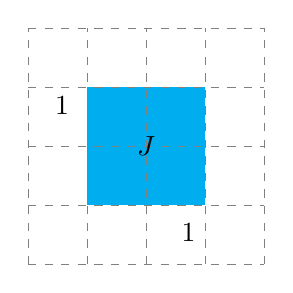
\begin{tikzpicture}[scale=0.75]
\fill[cyan] (0,0) rectangle (2,2);
\draw[help lines,dashed] (-1,-1) grid (3,3);
\node at (1,1) {$J$};
\gridlines{-1}{3}{-1}{3};
\node[below left, yshift=-3] at (2,0) {$1$};
\node[below left, xshift=-3] at (0,2) {$1$};
\end{tikzpicture}
\end{center}
\end{multicols}
\begin{enumerate}
%Phillip Goins
\begin{multicols}{2}
\item Multiplication by the matrix $\mtx{rr}{2&0\\0&1}$ horizontally stretches the plane by a factor of two. \\

\mbox{}\\
\begin{center}
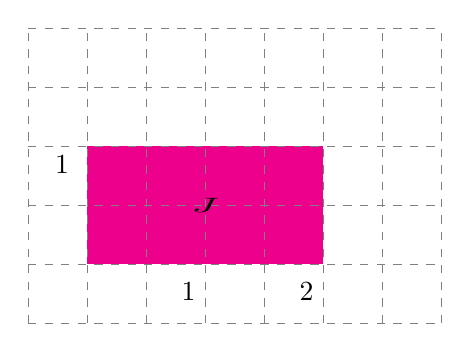
\begin{tikzpicture}[scale=0.75]
\fill[magenta] (0,0) rectangle (4,2);
\draw[help lines,dashed] (-1,-1) grid (6,4);
\begin{scope}[cm={2,0,0,1,(0,0)}]
\node[transform shape] at (1,1) {$J$};
\end{scope}
\gridlines{-1}{6}{-1}{4};
\node[below left, yshift=-3] at (2,0) {$1$};
\node[below left, yshift=-3] at (4,0) {$2$};
\node[below left, xshift=-3] at (0,2) {$1$};
%\node[below left, xshift=-3] at (0,4) {$2$};
%\node[below left, xshift=-3] at (0,6) {$3$};
\end{tikzpicture}
\end{center}
\end{multicols}

\begin{multicols}{2}
\item Multiplication by the matrix $\mtx{rr}{8&0\\0&1}$ horizontally stretches the plane by a factor of eight. \\

\mbox{}\\
\begin{center}
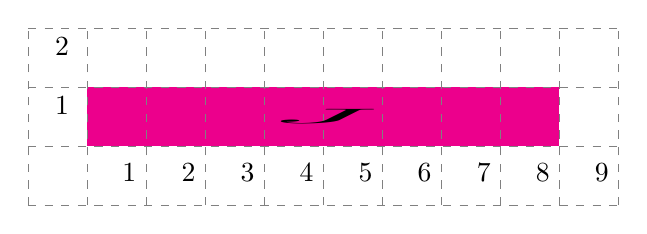
\begin{tikzpicture}[scale=0.75]
\fill[magenta] (0,0) rectangle (8,1);
\draw[help lines,dashed] (-1,-1) grid (9,2);
\begin{scope}[cm={8,0,0,1,(0,0)}]
\node[transform shape] at (0.5,0.5) {$J$};
\end{scope}
\gridlines{-1}{9}{-1}{2};
\node[below left, yshift=-3] at (1,0) {$1$};
\node[below left, yshift=-3] at (2,0) {$2$};
\node[below left, yshift=-3] at (3,0) {$3$};
\node[below left, yshift=-3] at (4,0) {$4$};
\node[below left, yshift=-3] at (5,0) {$5$};
\node[below left, yshift=-3] at (6,0) {$6$};
\node[below left, yshift=-3] at (7,0) {$7$};
\node[below left, yshift=-3] at (8,0) {$8$};
\node[below left, yshift=-3] at (9,0) {$9$};
\node[below left, xshift=-3] at (0,1) {$1$};
\node[below left, xshift=-3] at (0,2) {$2$};
\end{tikzpicture}
\end{center}
    
\end{multicols}\pagebreak

\begin{multicols}{2}
\item Multiplication by the matrix $\mtx{rr}{1&0\\0&4}$ vertically stretches the plane by a factor of four. \\

\mbox{}\\
\begin{center}
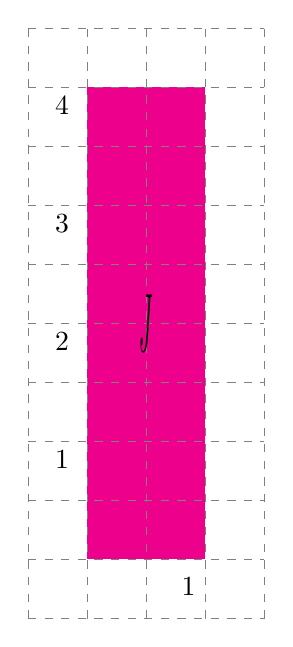
\begin{tikzpicture}[scale=0.75]
\fill[magenta] (0,0) rectangle (2,8);
\draw[help lines,dashed] (-1,-1) grid (3,9);
\begin{scope}[cm={1,0,0,4,(0,0)}]
\node[transform shape] at (1,1) {$J$};
\end{scope}
\gridlines{-1}{3}{-1}{9};
\node[below left, yshift=-3] at (2,0) {$1$};
\node[below left, xshift=-3] at (0,2) {$1$};
\node[below left, xshift=-3] at (0,4) {$2$};
\node[below left, xshift=-3] at (0,6) {$3$};
\node[below left, xshift=-3] at (0,8) {$4$};
\end{tikzpicture}
\end{center}
\end{multicols}

\begin{multicols}{2}
\item Multiplication by the matrix $\mtx{rr}{1&0\\0&\frac{1}{2}}$ vertically comprresses the plane by a factor of two. \\

\mbox{}\\
\begin{center}
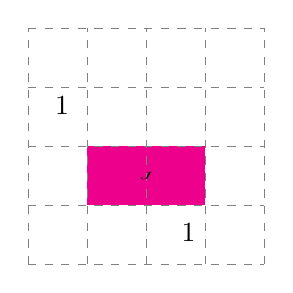
\begin{tikzpicture}[scale=0.75]
\fill[magenta] (0,0) rectangle (2,1);
\draw[help lines,dashed] (-1,-1) grid (3,3);
\begin{scope}[cm={1,0,0,0.5,(0,0)}]
\node[transform shape] at (1,1) {$J$};
\end{scope}
\gridlines{-1}{3}{-1}{3};
\node[below left, yshift=-3] at (2,0) {$1$};
\node[below left, xshift=-3] at (0,2) {$1$};
\end{tikzpicture}
\end{center}
\end{multicols}
\end{enumerate}
\end{Exam}

\begin{Exam} The matrix $\mtx{cc}{1/2&0\\0&3} = \mtx{cc}{\frac{1}{2}&0\\0&1}\mtx{rr}{1&0\\0&3}$ will vertically stretch the four vertices of $J$ by a factor of 3 and will horizontally compress the vertices by a factor of 2 (or we can say that they are horizontally stretched by a factor of 1/2). In particular, \vspace{-0.2 in}
\begin{multicols}{2}
\[\mtx{cc}{\frac{1}{2}&0\\0&3}\vr{0\\0} = \vr{0\\0}\]
\[\mtx{cc}{\frac{1}{2}&0\\0&3}\vr{1\\0} = \mtx{c}{\frac{1}{2}\\0}\]
\[\mtx{cc}{\frac{1}{2}&0\\0&3}\vr{0\\1} = \vr{0\\3}\]
\[\mtx{cc}{\frac{1}{2}&0\\0&3}\vr{1\\1} = \mtx{c}{\frac{1}{2}\\3}\]
The image of $J$ is displayed to the right in magenta.\columnbreak

\mbox{}\\
\begin{center}
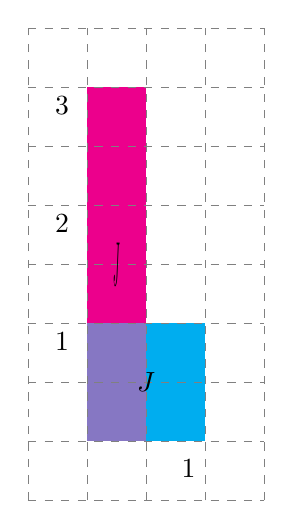
\begin{tikzpicture}[scale=0.75]
\fill[cyan] (0,0) rectangle (2,2);
\fill[magenta] (0,0) rectangle (1,6);
\fill[magenta!50!cyan] (0,0) rectangle (1,2);
\draw[help lines,dashed] (-1,-1) grid (3,7);
\node at (1,1) {$J$};
\begin{scope}[cm={0.5,0,0,3,(0,0)}]
\node[transform shape] at (1,1) {$J$};
\end{scope}
\gridlines{-1}{3}{-1}{7};
\node[below left, yshift=-3] at (2,0) {$1$};
\node[below left, xshift=-3] at (0,2) {$1$};
\node[below left, xshift=-3] at (0,4) {$2$};
\node[below left, xshift=-3] at (0,6) {$3$};
\end{tikzpicture}
\end{center}\hfill$\qedhere$
\end{multicols}
\end{Exam}

In plane geometry, a shear mapping (or transvection) is a linear map that displaces each point in fixed direction, by an amount proportional to its signed distance from a line that is parallel to that direction. Let $m\in \R$. \vspace{-0.1 in}
\begin{multicols}{2}
\noindent We can \textbf{shear} $\R^2$ \textbf{horizontally} by multiplying the (replacement) matrix 
\[\mtx{cc}{1&m\\0&1}.\] 
\noindent We can \textbf{shear} $\R^2$ \textbf{vertically} by multiplying the matrix 
\[\mtx{cc}{1&0\\m&1}.\]
\end{multicols} \vspace{-0.1 in}

\begin{Exam} Consider the shearing of the unit square and the points $\bb u = (2,1)$ and $\bb v= (1,2)$:
\begin{enumerate}
\begin{multicols}{2}
\item horizontally by a factor of $2$.\\

The images of these points under this shear are 
\[\mtx{rr}{1&2\\0&1}\vr{2\\1} = \vr{4\\1};\]
\[\mtx{rr}{1&2\\0&1}\vr{1\\2} = \vr{5\\2}.\] \vfill
\begin{center}
\begin{tikzpicture}[scale=0.75]
\fill[cyan] (0,0) rectangle (1,1);
\node at (0.5, 0.5) {$J$};
\fill[magenta] (0,0) -- (2,1) -- (3,1) -- (1,0) -- cycle;
\fill[magenta!50!cyan] (0,0) -- (1,0) -- (1,0.5) -- cycle;
\begin{scope}[cm={1,0,2,1,(0,0)}]
\node[transform shape] at (0.5,0.5) {$J$};
\end{scope}
\draw[help lines,dashed] (-1,-3) grid (5,3);
\gridlines{-1}{5}{-3}{3};
\draw[blue, ultra thick, dashed, ->] ($ (2,1) + (0.1,0) $) -- ($ (4,1) + (-0.1, 0) $);
\draw[blue, ultra thick, dashed, ->] ($ (1,2) + (0.1,0) $) -- ($ (5,2) + (-0.1, 0) $);
\fill[cyan] (2,1) circle (0.125) node[above] {$\bb u$};
\fill[magenta] (4,1) circle (0.125) node[above] {$\bb u'$};
\fill[cyan] (1,2) circle (0.125) node[above] {$\bb v$};
\fill[magenta] (5,2) circle (0.125) node[above] {$\bb v'$};
\end{tikzpicture}
\end{center}
\end{multicols}

\begin{multicols}{2}
\item vertically by a factor of $-2$.\\

The  images of $\bb u$ and $\bb v$ under this shear are 
\[\mtx{rr}{1&0\\-2&1}\vr{2\\1} = \vr{2\\-3};\]
\[\mtx{rr}{1&0\\-2&1}\vr{1\\2} = \vr{1\\0}.\]\vfill
\begin{center}
\begin{tikzpicture}[scale=0.75]
\fill[cyan] (0,0) rectangle (1,1);
\node at (0.5, 0.5) {$J$};
\fill[magenta] (0,0) -- (0,1) -- (1,-1) -- (1,-2) -- cycle;
\fill[magenta!50!cyan] (0,0) -- (0,1) -- (0.5,0) -- cycle;
\begin{scope}[cm={1,-2,0,1,(0,0)}]
\node[transform shape] at (0.5,0.5) {$J$};
\end{scope}
\draw[help lines,dashed] (-3,-3) grid (3,3);
\gridlines{-3}{3}{-3}{3};
\draw[blue, ultra thick, dashed, ->] ($ (2,1) + (0, -0.1) $) -- ($ (2,-3) + (0, 0.1) $);
\draw[blue, ultra thick, dashed, ->] ($ (1,2) + (0, 0.1) $) -- ($ (1,0) + (0,0.1) $);
\fill[cyan] (2,1) circle (0.125) node[right] {$\bb u$};
\fill[magenta] (2,-3) circle (0.125) node[right] {$\bb u'$};
\fill[cyan] (1,2) circle (0.125) node[right] {$\bb v$};
\fill[magenta] (1,0) circle (0.125) node[below right] {$\bb v'$};
\end{tikzpicture}
\end{center}\hfill$\qedhere$

\end{multicols}
\end{enumerate}
\end{Exam}


\begin{multicols}{2}
Reflections across the $x$- and $y$-axis are accomplished by multiplying by the scaling (diagonal) matrices 
\[\mtx{rr}{1&0\\0&-1} \quad \text{and}\quad  \mtx{rr}{-1&0\\0&1},\] respectively.\columnbreak
\mbox{}\\
\begin{center}
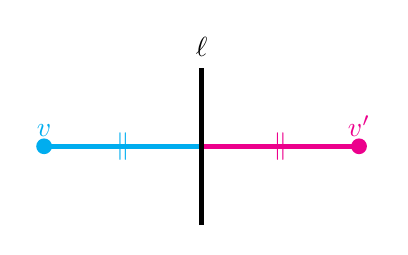
\begin{tikzpicture}
\draw[ultra thick, magenta] (0,0) -- (2,0) node[midway] {$\Vert$};
\draw[ultra thick, cyan] (0,0) -- (-2,0)  node[midway] {$\Vert$};
\draw[ultra thick] (0, -1) -- (0,1) node[above] {$\ell$};
\fill[magenta] (2,0) circle (0.1) node[above] {$\bb v'$};
\fill[cyan] (-2,0) circle (0.1) node[above] {$\bb v$};
\end{tikzpicture}
\end{center}
\end{multicols}\vspace{-0.2 in}
\noindent The interchange (permutation) matrix $\mtx{rr}{0&1\\1&0}$ produces a reflection across the line $y=x$. The composite of reflections across the $x$- and $y$-axis gives a reflection through the origin. General reflections will be discussed in the homework. \\


\begin{Exam} Consider the reflections of point $\bb v = (2,1)$ across:
\begin{enumerate}
\begin{multicols}{2}
\item the $x$-axis.\\

The image of $\bb v$ under this reflection is 
\[\mtx{rr}{1&0\\0&-1}\vr{2\\1} = \vr{2\\-1}.\] \vfill
\begin{center}
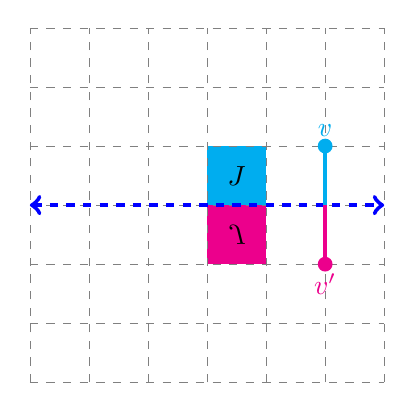
\begin{tikzpicture}[scale=0.75]
\fill[cyan] (0,0) rectangle (1,1);
\node at (0.5, 0.5) {$J$};
\fill[magenta] (0,0) rectangle (1,-1);
\node[yscale=-1] at (0.5, -0.5) {$J$};
\draw[help lines,dashed] (-3,-3) grid (3,3);
\gridlines{-3}{3}{-3}{3};
\draw[ultra thick, blue, <->, dashed] (-3,0) -- (3,0);
\fill[cyan] (2,1) circle (0.125) node[above] {$\bb v$};
\draw[cyan, ultra thick] (2,1) -- (2,0);
\draw[magenta, ultra thick] (2,0) -- (2,-1);
\fill[magenta] (2,-1) circle (0.125) node[below] {$\bb v'$};
\end{tikzpicture}
\end{center}
\end{multicols}

\begin{multicols}{2}
\item the $y$-axis.\\

The image of $\bb v$ under this reflection is 
\[\mtx{rr}{-1&0\\0&1}\vr{2\\1} = \vr{-2\\1}.\]\vfill
\begin{center}
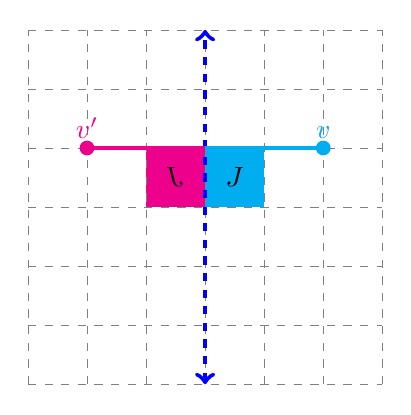
\begin{tikzpicture}[scale=0.75]
\fill[cyan] (0,0) rectangle (1,1);
\node at (0.5, 0.5) {$J$};
\fill[magenta] (0,0) rectangle (-1,1);
\node[xscale=-1] at (-0.5, 0.5) {$J$};
\draw[help lines,dashed] (-3,-3) grid (3,3);
\gridlines{-3}{3}{-3}{3};
\draw[ultra thick, blue, <->, dashed] (0,-3) -- (0,3);
\fill[cyan] (2,1) circle (0.125) node[above] {$\bb v$};
\draw[cyan, ultra thick] (2,1) -- (0,1);
\draw[magenta, ultra thick] (0,1) -- (-2,1);
\fill[magenta] (-2,1) circle (0.125) node[above] {$\bb v'$};
\end{tikzpicture}
\end{center}

\end{multicols}
\begin{multicols}{2}
\item $y=x$.\\

The image of $\bb v$ under this reflection is 
\[\mtx{rr}{0&1\\1&0}\vr{2\\1} = \vr{1\\2}.\]\vfill
\begin{center}
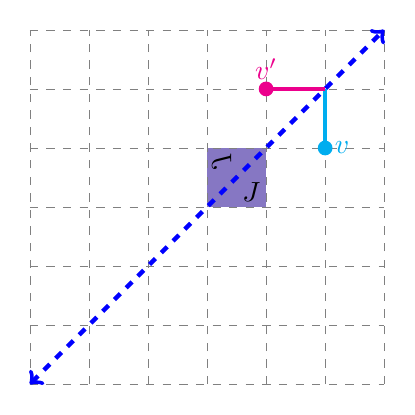
\begin{tikzpicture}[scale=0.75]
\fill[cyan!50!magenta] (0,0) rectangle (1,1);
\node at (0.75, 0.25) {$J$};
\node[xscale=-1, rotate=90] at (0.25, 0.75) {$J$};
\draw[help lines,dashed] (-3,-3) grid (3,3);
\gridlines{-3}{3}{-3}{3};
\draw[ultra thick, blue, <->, dashed] (-3,-3) -- (3,3);
\fill[cyan] (2,1) circle (0.125) node[right] {$\bb v$};
\draw[cyan, ultra thick] (2,1) -- (2,2);
\draw[magenta, ultra thick] (2,2) -- (1,2);
\fill[magenta] (1,2) circle (0.125) node[above] {$\bb v'$};
\end{tikzpicture}
\end{center}

\end{multicols}
\begin{multicols}{2}
\item the origin.\\

The image of $\bb v$ under this reflection is 
\[\mtx{rr}{-1&0\\0&-1}\vr{2\\1} = \vr{-2\\-1}.\]\vfill
\begin{center}
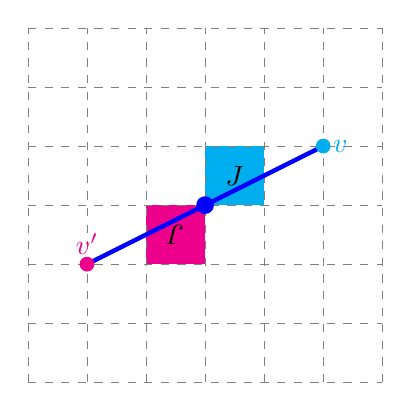
\begin{tikzpicture}[scale=0.75]
\fill[cyan] (0,0) rectangle (1,1);
\node at (0.5, 0.5) {$J$};
\fill[magenta] (0,0) rectangle (-1,-1);
\node[yscale=-1, xscale=-1] at (-0.5, -0.5) {$J$};
\draw[help lines,dashed] (-3,-3) grid (3,3);
\gridlines{-3}{3}{-3}{3};
\draw[blue, ultra thick] (2,1) -- (0,0);
\draw[blue, ultra thick] (0,0) -- (-2,-1);
\fill[cyan] (2,1) circle (0.125) node[right] {$\bb v$};
\fill[magenta] (-2,-1) circle (0.125) node[above] {$\bb v'$};
\fill[blue] (0,0) circle (0.15);
\end{tikzpicture}
\end{center}\hfill$\qedhere$

\end{multicols}
\end{enumerate}
\end{Exam}

\begin{Thm}\label{thm:elementarymatrixtransform} Let $A$ be a $2\times 2$ nonsingular matrix. Then the matrix transformation associated to $A$ geometrically is a composition of shears, reflections, and stretches/compressions. 
\end{Thm}

The following example illustrates \thmref{thm:elementarymatrixtransform}.

\begin{Exam} %Skyler Clark
Let $A=\mtx{rr}{-4&-5\\2&4}$. We reduce $A$ to its row reduced echelon form in the following way:
\[\begin{tikzpicture}
\path (0,0) node {$\mtx{rr}{-4&-5\\2&4}\quad \sim \mtx{rr}{2\phantom{\Big.^{\color{red}\ 4}}&4\phantom{\Big.^{\color{red}\ 8}}\\
-4{\Big.^{\color{red}\ 4}}&-5{\Big.^{\color{red}\ 8}}
} 
%
\hspace{-7 pt}\begin{array}{c} \mbox{} \\ \color{red} \footnotesize  (\text{Row 2 + 2 Row 1}) \end{array} 
%
\sim \mtx{rr}{\color{red}{\Big.^{\color{red}\ 1}}\cancel{\color{black}2}&\color{red}{\Big.^{\color{red}\ 2}}\cancel{\color{black}4}\\0&3} \hspace{-7 pt}\begin{array}{c} \color{red} \footnotesize  \Big(\frac{1}{2}\text{Row 1}\Big) \\ \mbox{} \end{array}
%
\sim \mtx{rr}{1&2\\0&\color{red}{\Big.^{\color{red}\ 1}}\cancel{\color{black}3}} \hspace{-7 pt}\begin{array}{c}   \mbox{} \\ \color{red} \footnotesize\Big(\frac{1}{3}\text{Row 2}\Big) \end{array}$};

\path (0,-2) node {$\mtx{rr}{
1&2{\Big.^{\color{red}\ -2}}\\
0&1\phantom{\Big.^{\color{red}\ -2}}}
\hspace{-7 pt}\begin{array}{c} \color{red} \footnotesize  (\text{Row 1 - 2 Row 2}) \\ \mbox{} \end{array} \sim \mtx{rr}{1&0\\0&1} $};
\begin{scope}[tips=proper]
\draw[ultra thick, red, stealth-stealth] (-6,-0.45) edge[bend right] (-6,0.45);
\end{scope}
\end{tikzpicture} \]
Following this sequence of row operation gives the following elementary factorization of $A$:
\[A = \mtx{rr}{0&1\\1&0}\mtx{rr}{1&0\\-2&1}\mtx{rr}{2&0\\0&1}\mtx{rr}{1&0\\0&3}\mtx{rr}{1&2\\0&1}.\] To translate this elementary factorization into a geometric interpretation, we read the factorization right-to-left. Why? Because with the transformation $\bb x \mapsto A\bb x = (E_1E_2E_3E_4E_5)\bb x$, assuming $E_i$ denotes the $i$th elementary factor in the above factorization of $A$, the first matrix to transform $\bb x$ will be $E_5$. The next to transform the resultant vector would be $E_4$, and onward toward the left. Hence, multiplication by $A$ has the affect of shearing horizontally by a factor of 2, stretching vertically by a factor of 3, stretching horizontally by a factor of 2, shearing vertically by a factor of $-2$, and reflecting across the diagonal line $y=x$. 
\end{Exam}

\begin{Exam} Let $A = \mtx{rr}{0&1\\2&1}$. We can row reduce $A$ by interchanges Rows 1 and 2, scaling Row 1 by $\frac{1}{2}$, and replacing Row 1 with $\row 1 - \frac{1}{2}\row 2$. This gives the following factorization into elementary matrices as
\[A = \mtx{rr}{0&1\\1&0}\mtx{rr}{2&0\\0&1}\mtx{cc}{1&1/2\\0&1}.\] Therefore, $A$ corresponds to the transformation shear horizontally by $\frac{1}{2}$, horizontally stretch by 2, and reflect across the line $y=x$.
\end{Exam}

\begin{multicols}{2}
A counterclockwise rotation in $\R^2$ by angle $\theta$ is captured by the matrix \[\mtx{rr}{\cos\theta &  -\sin\theta\\ \sin \theta & \cos \theta}.\] 

\begin{center}
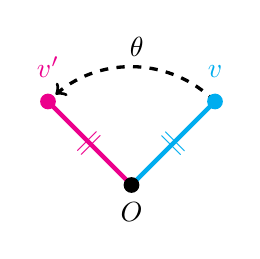
\begin{tikzpicture}
\draw[very thick, dashed, ->] (45:1.5) arc(45:130:1.5) node[midway,,above] {$\theta$};
\fill[cyan] (45:1.5) circle (0.1) coordinate (P) node[above, yshift=5] {$\bb v$};
\fill[magenta] (135:1.5) circle (0.1) coordinate (P')  node[above, yshift=5] {$\bb v'$};
\draw[ultra thick, magenta] (0,0) -- (P') node[midway, sloped] {$\Vert$};
\draw[ultra thick, cyan] (0,0) -- (P)  node[midway, sloped] {$\Vert$};
\fill (0,0) circle (0.1) node[below, yshift=-3] {$O$}; 
\end{tikzpicture}
\end{center}
\end{multicols}\vspace{-0.1 in}
\noindent For a clockwise rotation by $\theta$, take the previous matrix's inverse, $\mtx{rr}{\cos\theta &  -\sin\theta\\ \sin \theta & \cos \theta}^{-1} = \mtx{rr}{\cos\theta &  \sin\theta\\ -\sin \theta & \cos \theta}$.\\

\begin{Exam} Let $T : \R^2 \to \R^2$ be the linear transformation given as counterclockwise rotation by $\dfrac{\pi}{2}$ (or $90^\circ$). Find the images under $T$ of $\bb u = \vr{4\\1}$, $\bb v = \vr{2\\3}$, and $\bb u + \bb v = \vr{6\\4}$.%\vspace{-0,25 in}
\begin{multicols}{2}
Note that $[T] = \mtx{rr}{0&-1\\1&0}$. Then
\begin{eqnarray*}
T(\bb u) &=& \mtx{rr}{0 & -1 \\ 1 & 0}\vr{4\\1} = \vr{-1\\4}\\
T(\bb v) &=& \mtx{rr}{0 & -1 \\ 1 & 0}\vr{2\\3} = \vr{-3\\2}\\
T(\bb u+\bb v) &=& \mtx{rr}{0 & -1 \\ 1 & 0}\vr{6\\4} = \vr{-4\\6}%\\
%& =&  \vr{-1\\4} +\vr{-3\\2}. 
\end{eqnarray*} \vfill

\begin{center}
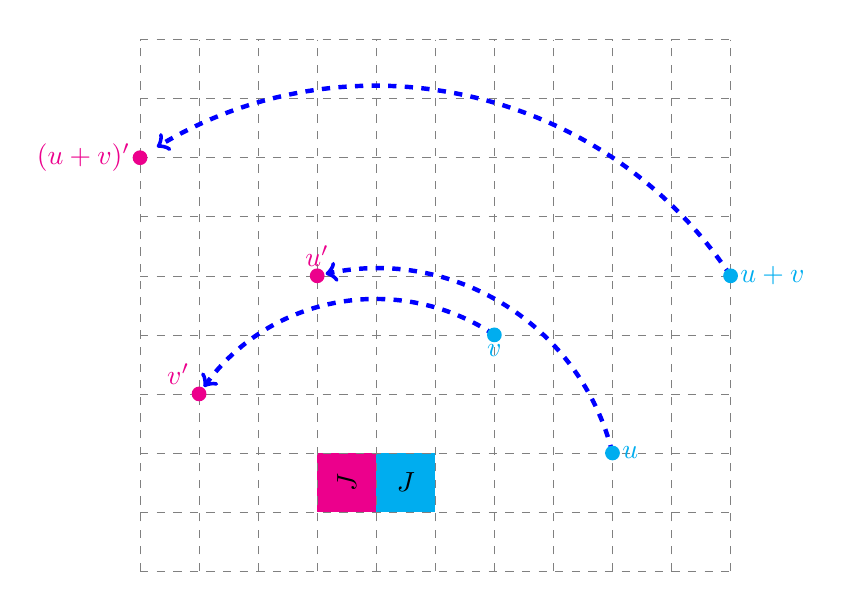
\begin{tikzpicture}[scale=0.75]
\fill[cyan] (0,0) rectangle (1,1);
\node at (0.5, 0.5) {$J$};
\fill[magenta] (0,0) rectangle (-1,1);
\node[rotate=90] at (-0.5, 0.5) {$J$};
\draw[help lines,dashed] (-4,-1) grid (6,8);
\gridlines{-4}{6}{-1}{8};
\draw[blue, ultra thick, ->, dashed] (4,1) arc(14.036:102:4.123);
\draw[blue, ultra thick, ->, dashed] (2,3) arc(56.310:144:3.606);
\draw[blue, ultra thick, ->, dashed] (6,4) arc(33.690:121:7.211);
\fill[cyan] (4,1) circle (0.125) node[right] {$\bb u$};
\fill[magenta] (-1,4) circle (0.125) node[above] {$\bb u'$};
\fill[cyan] (2,3) circle (0.125) node[below] {$\bb v$};
\fill[magenta] (-3,2) circle (0.125) node[above left] {$\bb v'$};
\fill[cyan] (6,4) circle (0.125) node[right] {$\bb u+\bb v$};
\fill[magenta] (-4,6) circle (0.125) node[left] {$(\bb u+\bb v)'$};
\end{tikzpicture}
\end{center}\hfill$\qedhere$
\end{multicols}
\end{Exam}
A similar analysis may be used to describe the geometry of matrix transformation in $\R^3$ (and higher).

%%%%%%%%%%%%%%%%%% Exercises %%%%%%%%%%%%%%%%%%%
\startExercises{trans2}

\noindent For Exercises \ref{exer:matrixgeostart}-\ref{exer:matrixgeostop}, find the matrix for the operator that performs the stated succession of geometric transformations.
\begin{enumerate}[!HW!, start=1, label=$\spadesuit$ \arabic*., ref=\arabic*]
\item\label{exer:matrixgeostart} Compress by a factor of 2 in the $x$-direction, then expands by a factor of $5$ in the $y$-direction. %Anton 4.11.7(a) p. 287
\itemspade Expands by a factor of $5$ in the $y$-direction, then shears by a factor of $2$ in the $y$-direction.%Anton 4.11.7(b) p. 287
\itemspade Reflects about $y=x$, then rotates through an angle of $\pi$ radians about the origin.%Anton 4.11.7(c) p. 287
\itemspade Reflects about the $y$-axis, then expands by a factor of 5 in the $x$-direction, and then reflects about $y=x$.%Anton 4.11.8(a) p. 287
\item\label{exer:matrixgeostop} Rotates through $\dfrac{\pi}{6}$ about the origin, then shears by a factor of $-2$ in the $y$-direction, and then expands by a factor of 3 in the $y$-direction.%Anton 4.11.8(b) p. 287
\end{enumerate}

\noindent For Exercises \ref{exer:matrixfactorgeostart}-\ref{exer:matrixfactorgeostop}, express the matrix as a product of elementary matrices, and then describe the effect of multiplication by this matrix in terms of shears, compressions/stretches, and reflections. Draw the image of the unit square under this matrix transformation. Answers may vary.
\begin{enumerate}[!HW!, label=$\spadesuit$ \arabic*., ref=\arabic*]
\begin{multicols}{4}
\item\label{exer:matrixfactorgeostart} $\mtx{rr}{4&0\\0&1}$ %Devan Hill
\itemspade $\mtx{rr}{1&0\\0&-8}$%Devan Hill
\itemspade $\mtx{rr}{0&-2\\4&0}$%Anton 4.11.11 p. 287
\item\label{exer:matrixfactorgeostop} $\mtx{rr}{3&-6\\6&1}$%Kennedy Worthington
\end{multicols}
\end{enumerate}

\begin{enumerate}[!HW!]
\item What matrix, if multiplied by, would have the affect to the plane $\R^2$ of reflection across the line $y=-x$? How could you factor this matrix using the matrix transformation discussed in this section?

\itemspade Let $A = \mtx{rr}{\cos 2\theta & \sin 2\theta \\ \sin 2\theta & -\cos 2\theta}$, where $\theta >0$.
\begin{enumerate}
\item Show that $A = \mtx{rr}{\cos \theta & -\sin \theta \\ \sin \theta & \cos \theta}\mtx{rr}{1 & 0 \\ 0 & -1}\mtx{rr}{\cos \theta & -\sin \theta \\ \sin \theta & \cos \theta}^{-1}$.
\item For $\mtx{rr}{\cos \theta & -\sin \theta \\ \sin \theta & \cos \theta}\mtx{rr}{1 & 0 \\ 0 & -1}\mtx{rr}{\cos \theta & -\sin \theta \\ \sin \theta & \cos \theta}^{-1}$ describe the sequence of geometric transformations that correspond to this matrix factorization. Conclude that the geometric transformation corresponding to $A$ is reflection across the line $\ell$ through the origin which forms an angle $\theta$ with the $x$-axis.
\item For $\theta=0$, $\dfrac{\pi}{4}$, and $\dfrac{\pi}{2}$, show that this agrees with the three reflections discussed in this section.
\item For $\theta = \dfrac{\pi}{6}$, compute the reflection matrix and draw the image of the unit square under this matrix transformation.
\item Modifying part (b), find a $2\times 2$ matrix $B$ where multiplication by $B$ performs the geometric transformation of shearing by a factor of $m$ in the direction of the line $\ell$ through the origin which forms an angle $\theta$ with the $x$-axis.
\end{enumerate}

\item Prove \thmref{thm:elementarymatrixtransform}.
\end{enumerate}


%%%%%%%%%%%%%%%%%%% Footnotes %%%%%%%%%%%%%%%%%%%
 \mbox{}\vfill
 \pagebreak